% ============================================================
% CHAPITRE 3 : COMPREHENSION ET PREPARATION DES DONNEES
% CRISP-DM - PHASES 2 et 3 (Data Understanding / Data Preparation)
% Structure canonique :
%   Phase 2 : collecte / description / exploration / verification qualite
%   Phase 3 : selection / nettoyage / construction / integration / formatage
%
% Figures : docs/rapport/img/fig_*.png  (generees par figures.py)
% Bibliographie : docs/rapport/references.bib
% ============================================================

\chapter{Compréhension et préparation des données}
\label{chap:donnees}
\minitocsection
\newpage

% ------------------------------------------------------------
\section*{Introduction}
\addcontentsline{toc}{section}{Introduction}
% ------------------------------------------------------------

Le chapitre précédent a clos la première phase de CRISP-DM en traduisant sept objectifs métier en huit objectifs de fouille de données, chacun assorti d'une métrique et d'un critère de succès. Ces objectifs ont été formulés à partir de la connaissance du domaine, sans que les données aient encore été examinées en détail. Le présent chapitre conduit les deuxième et troisième phases du cycle : il confronte ces objectifs à la réalité des sources disponibles, puis construit le jeu de données à partir duquel la modélisation sera possible.

Cette confrontation est le moment de vérité méthodologique de la démarche. Un objectif analytique qui paraît raisonnable en réunion peut se révéler inatteignable dès lors que l'on mesure la profondeur d'historique réellement disponible, la proportion de références dont les ventes sont trop rares pour porter une saisonnalité, ou la fiabilité des identifiants qui relient deux domaines métier. CRISP-DM prévoit explicitement cette boucle de retour : la phase de compréhension des données peut conduire à réviser la formulation du problème \cite{chapman2000crisp}. Nous verrons que ce cas s'est effectivement présenté et que deux objectifs ont dû voir leur périmètre resserré.

Les phases 2 et 3 sont traitées dans un même chapitre parce qu'elles partagent les mêmes sources et s'entremêlent dans la pratique : on ne découvre certaines anomalies qu'en tentant de construire une variable, et l'on ne mesure la portée d'un défaut de qualité qu'en observant son effet sur un agrégat. Les traiter séparément aurait imposé des allers-retours artificiels entre deux chapitres.

Le chapitre suit l'ordre canonique des tâches génériques de CRISP-DM. La section~\ref{sec:collecte} décrit la collecte des données initiales et la volumétrie obtenue. La section~\ref{sec:description} en donne la description structurelle : organisation en schémas métier, dictionnaire de données, modèle relationnel. La section~\ref{sec:exploration} présente l'exploration statistique, dont les résultats orientent directement les choix de modélisation du chapitre~\ref{chap:modelisation}. La section~\ref{sec:qualite} rend compte de la vérification de la qualité, avec le relevé exhaustif des anomalies constatées et leur traitement. La section~\ref{sec:preparation} détaille la préparation proprement dite, décomposée en ses cinq tâches. La section~\ref{sec:jeu-final} décrit enfin le jeu de données final et le protocole de découpage temporel qui garantit l'absence de fuite d'information.

% ------------------------------------------------------------
\section{Collecte des données initiales}
\label{sec:collecte}
% ------------------------------------------------------------

\subsection{Sources mobilisées et mode d'acquisition}

Le système exploite quatre familles de sources, de nature et de fraîcheur très différentes. Cette hétérogénéité est structurante : elle explique une grande partie des choix d'architecture de données décrits plus loin.

La \textbf{première famille} est l'historique commercial, fourni sous forme d'extractions du système de caisse des points de vente. Ces extractions couvrent la ligne de ticket : un enregistrement par produit vendu, avec la boutique, le conseiller, l'horodatage, la quantité et les montants. C'est la source la plus volumineuse et la seule qui porte une profondeur d'historique suffisante pour l'apprentissage de saisonnalités.

La \textbf{deuxième famille} est le flux de ventes en temps réel. Contrairement à l'historique, il ne s'agit pas d'une extraction périodique mais d'un flux continu, alimenté transaction par transaction. Ce flux est indispensable au coaching : c'est lui qui permet de connaître la position de caisse d'une boutique à l'instant présent, donc de mesurer un écart à l'objectif en cours de journée. Sa contrepartie est une exigence de tolérance : le flux ne doit jamais être bloqué par un enregistrement incomplet, ce qui impose des contraintes d'intégrité volontairement plus permissives que sur l'historique.

La \textbf{troisième famille} regroupe les données de stock et d'approvisionnement : niveaux de stock par référence et par point de vente, instantanés historiques, mouvements, fournisseurs, catalogue de sourcing et bons de commande. Ces données sont acquises par extraction périodique et présentent une granularité temporelle plus grossière que les ventes.

La \textbf{quatrième famille} rassemble les signaux de contexte : calendrier des jours fériés et des fêtes religieuses, événements nationaux et locaux datés et géolocalisés, prix relevés chez les concurrents, motifs saisonniers, données météorologiques. Ces signaux proviennent de sources externes hétérogènes, certains par appel à des services de données ouvertes, d'autres par constitution manuelle d'un référentiel. Ils sont peu volumineux mais déterminants pour la qualité des prévisions, comme le montrera le chapitre~\ref{chap:evaluation}.

\subsection{Périmètre retenu}

Le périmètre de collecte a été arrêté en cohérence avec le périmètre projet défini au chapitre~\ref{chap:cadre-general}. Il porte sur l'ensemble du réseau de points de vente, sur une profondeur d'historique de vingt-deux mois, et à deux granularités temporelles simultanées : la granularité journalière, nécessaire à la prévision de la demande et à la mesure des saisonnalités, et la granularité horaire, nécessaire à la détection des heures de sous-performance visée par l'objectif OD-2.

Le choix d'une double granularité mérite d'être justifié car il double le coût de préparation. Une granularité uniquement journalière aurait suffi au domaine des stocks mais aurait rendu OD-2 inatteignable : détecter qu'une heure est anormale suppose de disposer d'un profil horaire attendu, lui-même appris sur l'historique horaire. Inversement, conserver toute la profondeur d'historique à la maille horaire pour le domaine des stocks aurait multiplié la volumétrie sans bénéfice, la demande de réapprovisionnement se raisonnant en jours. Les deux granularités coexistent donc, la seconde étant dérivée de la première par agrégation.

\subsection{Volumétrie obtenue}

La base constituée est une base PostgreSQL nommée \texttt{ooredoo\_sales}, d'un volume d'environ un gigaoctet, organisée en neuf schémas logiques et comptant cinquante et une tables et seize vues. Le tableau~\ref{tab:volumetrie-chap3} donne la volumétrie des principales tables et la période qu'elles couvrent.

\begingroup
\setlength{\tabcolsep}{3pt}
\renewcommand{\arraystretch}{1.15}
\small

\begin{longtable}{|P{4.6cm}|P{2.4cm}|P{3.0cm}|P{4.2cm}|}
\hline
\rowcolor{red!75}
\textcolor{white}{\textbf{Table}} &
\textcolor{white}{\textbf{Volumétrie}} &
\textcolor{white}{\textbf{Période couverte}} &
\textcolor{white}{\textbf{Objectifs servis}} \\
\hline
\endhead
\hline
\endfoot
\hline
\endlastfoot
Transactions historiques & 1{,}93 M lignes & oct. 2024 -- juil. 2026 & OD-1, OD-2, OD-3, OD-6 \\
\hline
Historique de stock & 1{,}12 M lignes & janv. 2025 -- juil. 2026 & OD-4 \\
\hline
Ventes agrégées par jour & 694 000 lignes & oct. 2024 -- juil. 2026 & OD-3, OD-5 \\
\hline
Exécutions d'agents & 127 000 lignes & courant projet & OD-8 \\
\hline
Indicateurs journaliers par conseiller & 114 000 lignes & déc. 2025 -- juil. 2026 & OD-6 \\
\hline
Objectifs commerciaux & 23 500 lignes & période projet & OD-1, OD-2 \\
\hline
Transactions temps réel & 9 500 lignes & flux continu & OD-1, OD-2 \\
\hline
Catalogue produits & 4 593 références \newline \small dont 2 277 actives & référentiel & OD-3 à OD-6 \\
\hline
Référentiel points de vente & 201 boutiques & référentiel & tous \\
\hline
Référentiel conseillers & 687 conseillers & référentiel & OD-6 \\
\hline
\caption{Volumétrie des principales tables et objectifs analytiques servis}
\label{tab:volumetrie-chap3}
\end{longtable}
\endgroup

Deux observations se dégagent de ce tableau et pèseront sur toute la suite. D'une part, le rapport entre le référentiel produit et le catalogue effectivement écoulé est très déséquilibré : sur les 4 593 références du catalogue, \textbf{572 seulement ont fait l'objet d'au moins une vente} sur la période, soit 12,5 \%. Les 87,5 \% restantes sont des références de catalogue sans mouvement observé : aucun modèle de prévision ne peut être construit pour elles, et la question n'est pas de savoir comment les prévoir mais de reconnaître qu'elles ne relèvent pas de la prévision. C'est le premier fait qui contraint la modélisation de l'objectif OD-3, et l'exploration en section~\ref{sec:exploration} montrera que la concentration se poursuit à l'intérieur même de ces 572 références.

L'activité observée porte par ailleurs sur 156 points de vente et 98 883 couples jour-boutique, ce qui fixe l'ordre de grandeur du panel disponible pour la prévision du chiffre d'affaires.

D'autre part, la profondeur d'historique de vingt-deux mois permet d'observer chaque saisonnalité annuelle majeure -- Ramadan, rentrée scolaire, fêtes de fin d'année -- une fois complètement et une seconde fois partiellement. C'est suffisant pour capturer une saisonnalité hebdomadaire de façon robuste, insuffisant pour estimer une composante annuelle avec confiance. Ce constat a conduit à écarter, dès cette phase, les modèles à composante annuelle explicite, et à privilégier une représentation des effets calendaires par variables exogènes plutôt que par décomposition saisonnière annuelle.

% ------------------------------------------------------------
\section{Description des données}
\label{sec:description}
% ------------------------------------------------------------

\subsection{Organisation en schémas métier}

Plutôt que de rassembler toutes les tables dans un espace unique, la base est organisée en neuf schémas logiques correspondant chacun à un domaine métier. Cette organisation n'est pas cosmétique : elle matérialise dans la structure de la base la séparation des domaines qui sera reprise dans l'architecture logicielle du chapitre~\ref{chap:modelisation}, et elle permet de raisonner sur les dépendances entre domaines en observant simplement les clés étrangères qui traversent les frontières de schéma. Le tableau~\ref{tab:schemas-chap3} présente ces neuf espaces.

\begingroup
\setlength{\tabcolsep}{3pt}
\renewcommand{\arraystretch}{1.15}
\small

\begin{longtable}{|P{2.2cm}|P{5.2cm}|P{6.6cm}|}
\hline
\rowcolor{red!75}
\textcolor{white}{\textbf{Schéma}} &
\textcolor{white}{\textbf{Domaine couvert}} &
\textcolor{white}{\textbf{Contenu principal}} \\
\hline
\endhead
\hline
\endfoot
\hline
\endlastfoot
\texttt{sales} & Référentiel commercial et ventes & Points de vente, conseillers, catalogue produit, transactions historiques et temps réel, objectifs \\
\hline
\texttt{inventory} & Stocks et pilotage & Ventes agrégées par jour, niveaux de stock, historique de stock, prévisions de demande, alertes, recommandations, exécutions d'agents \\
\hline
\texttt{supply} & Approvisionnement & Fournisseurs, catalogue de sourcing, bons de commande, mouvements de stock, transferts inter-boutiques \\
\hline
\texttt{market} & Contexte marché & Concurrents et prix relevés, événements nationaux datés, flux de portabilité, motifs saisonniers \\
\hline
\texttt{customer} & Voix du client & Segments de clientèle, enquêtes de satisfaction \\
\hline
\texttt{coaching} & Séances de coaching & Trace détaillée des interactions générées par les agents \\
\hline
\texttt{monitoring} & Observabilité & Vues de supervision uniquement, aucune table propre \\
\hline
\texttt{public} & Transverse & Comptes et sessions, indicateurs agrégés, journalisation des agents, validation humaine, boucle de retour, télémétrie de la recherche documentaire \\
\hline
\caption{Organisation de la base en schémas métier}
\label{tab:schemas-chap3}
\end{longtable}
\endgroup

\subsection{Dictionnaire des données principales}

Le tableau~\ref{tab:dictionnaire-chap3} donne le dictionnaire des attributs les plus structurants, c'est-à-dire ceux qui sont directement consommés par au moins un objectif analytique. Le dictionnaire complet, table par table et colonne par colonne, est reporté en annexe.

\begingroup
\setlength{\tabcolsep}{3pt}
\renewcommand{\arraystretch}{1.15}
\small

\begin{longtable}{|P{3.3cm}|P{2.0cm}|P{5.0cm}|P{3.6cm}|}
\hline
\rowcolor{red!75}
\textcolor{white}{\textbf{Attribut}} &
\textcolor{white}{\textbf{Type}} &
\textcolor{white}{\textbf{Signification}} &
\textcolor{white}{\textbf{Usage analytique}} \\
\hline
\endhead
\hline
\endfoot
\hline
\endlastfoot
Identifiant boutique & Texte & Clé du point de vente & Clé de partitionnement de toutes les séries \\
\hline
Référence produit & Entier & Clé du catalogue & Maille de la prévision de demande \\
\hline
Horodatage de vente & Horodatage & Instant de la transaction & Dérivation du jour et de l'heure \\
\hline
Quantité vendue & Entier & Unités cédées & Cible de la prévision de demande (OD-3) \\
\hline
Montant toutes taxes & Numérique & Valeur de la ligne & Cible de la prévision de CA (OD-1) \\
\hline
Marge & Numérique & Marge de la ligne & Critère de hiérarchisation produit (OD-6) \\
\hline
Délai de livraison moyen & Entier (jours) & Délai fournisseur attendu & Point de commande, stock de sécurité (OD-5) \\
\hline
Écart-type du délai & Entier (jours) & Variabilité du délai & Stock de sécurité (OD-5) \\
\hline
Quantité minimale de commande & Entier & Contrainte fournisseur & Arrondi de la quantité recommandée (OD-5) \\
\hline
Coût de possession & Pourcentage & Coût annuel de détention & Quantité économique de commande (OD-5) \\
\hline
Coût de passation & Numérique & Coût fixe d'une commande & Quantité économique de commande (OD-5) \\
\hline
Étape du cycle de vie & Texte & Lancement, croissance, maturité, déclin, fin de vie & Ajustement du niveau de service (OD-5) \\
\hline
Quantité en stock & Entier & Stock physique disponible & Classification du risque (OD-4) \\
\hline
Objectif de chiffre d'affaires & Numérique & Cible journalière du point de vente & Référence de l'écart (OD-1, OD-2) \\
\hline
Date et portée d'événement & Date, géo & Événement national ou local daté & Variable exogène de contexte (OD-3) \\
\hline
\caption{Dictionnaire des attributs structurants et de leur usage analytique}
\label{tab:dictionnaire-chap3}
\end{longtable}
\endgroup

Ce tableau appelle un commentaire méthodologique. Les six derniers attributs de la liste -- délais, coûts, contraintes fournisseurs, cycle de vie -- ne sont pas des données observées mais des \textit{paramètres de gestion} : ils décrivent des règles de l'entreprise et non des faits mesurés. Leur qualité ne se vérifie donc pas par des statistiques descriptives mais par confrontation aux pratiques réelles des approvisionneurs. Cette vérification a révélé que ces paramètres sont, pour une large part du catalogue, laissés à leur valeur par défaut. La conséquence est directe et sera assumée au chapitre~\ref{chap:evaluation} : la précision des quantités recommandées est bornée par la qualité de ces paramètres, non par celle du modèle de décision.

\subsection{Modèle relationnel}

La figure~\ref{fig:schema-relationnel-chap3} présente le modèle relationnel restreint aux entités centrales et aux relations qui traversent les frontières de domaine. Le modèle complet, qui comporte cinquante et une tables, est reporté en annexe.

\begin{figure}[H]
    \centering
    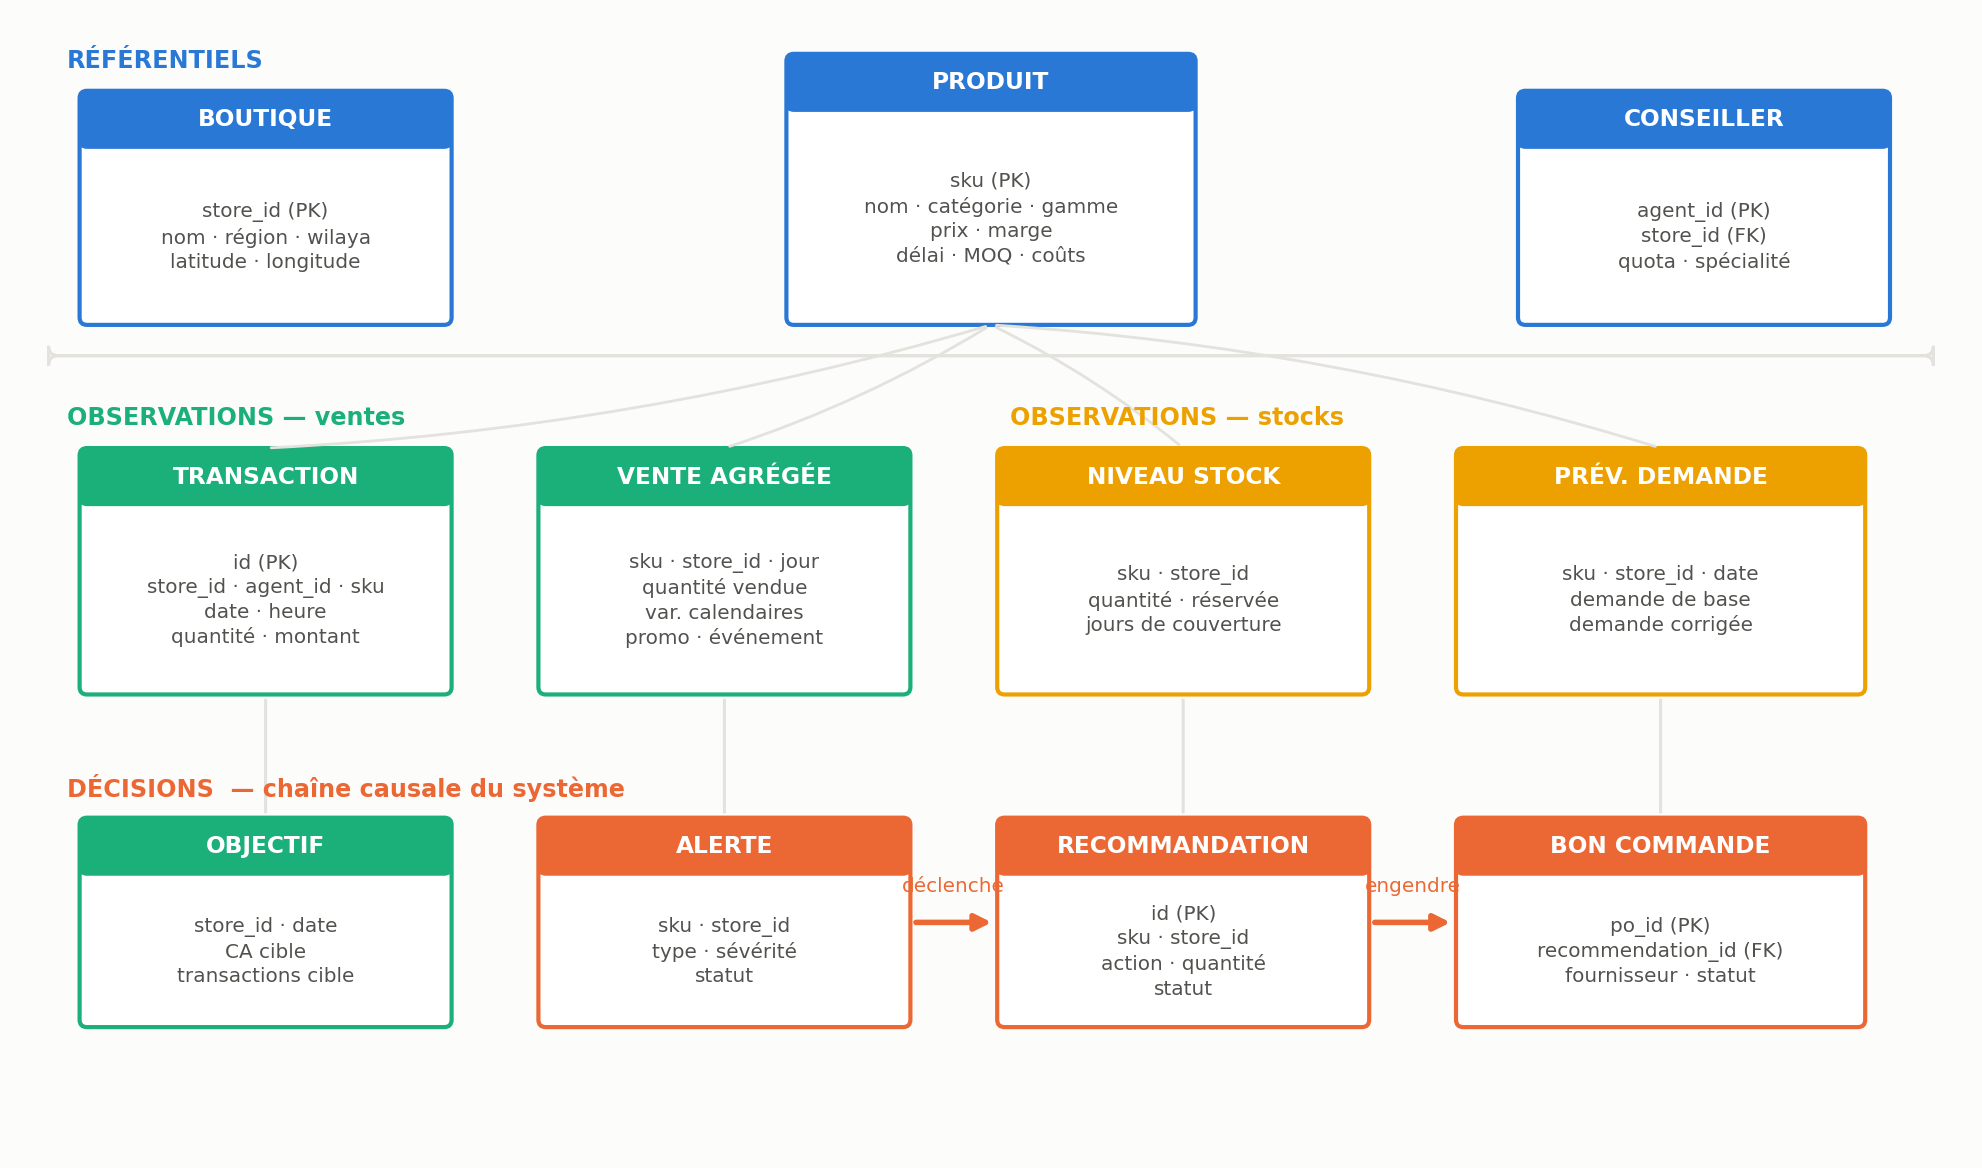
\includegraphics[width=\textwidth]{img/fig_schema_relationnel.png}
    \caption{Modèle relationnel des entités centrales et des relations inter-domaines}
    \label{fig:schema-relationnel-chap3}
\end{figure}

Trois tables de référence -- points de vente, catalogue produit et conseillers -- concentrent l'essentiel des clés étrangères de la base : quatorze tables se rattachent au référentiel des points de vente et treize au catalogue produit. Cette structure en étoile autour d'un noyau de référentiels est ce qui rend possible le croisement des deux domaines métier au cœur du projet : une recommandation de vente et une décision de réapprovisionnement portent sur le même couple point de vente et référence, ce qui autorise le raisonnement conjoint que l'objectif OD-6 exige.

La relation la plus significative pour la suite est celle qui relie une recommandation approuvée au bon de commande qu'elle engendre. Elle matérialise dans le modèle de données la chaîne causale complète : une anomalie détectée produit une alerte, l'alerte déclenche une analyse, l'analyse produit une recommandation, la recommandation validée par un responsable devient un bon de commande, et le bon de commande reçu met à jour le stock. Sans cette relation explicite, il serait impossible d'évaluer a posteriori la qualité des décisions du système, ce que l'objectif OD-5 réclame par son critère de succès -- le taux d'acceptation des propositions.

% ------------------------------------------------------------
\section{Exploration des données}
\label{sec:exploration}
% ------------------------------------------------------------

L'exploration poursuit un but précis : vérifier que les régularités supposées lors de la formulation des objectifs analytiques existent effectivement dans les données. Chaque analyse présentée ci-dessous est donc rattachée à l'objectif dont elle conditionne la faisabilité.

\subsection{Profil intra-journalier du chiffre d'affaires}

L'objectif OD-2 suppose qu'il existe un profil horaire attendu, suffisamment stable pour qu'un écart à ce profil constitue un signal exploitable. La figure~\ref{fig:profil-horaire-chap3} présente la distribution du chiffre d'affaires par heure d'ouverture.

\begin{figure}[H]
    \centering
    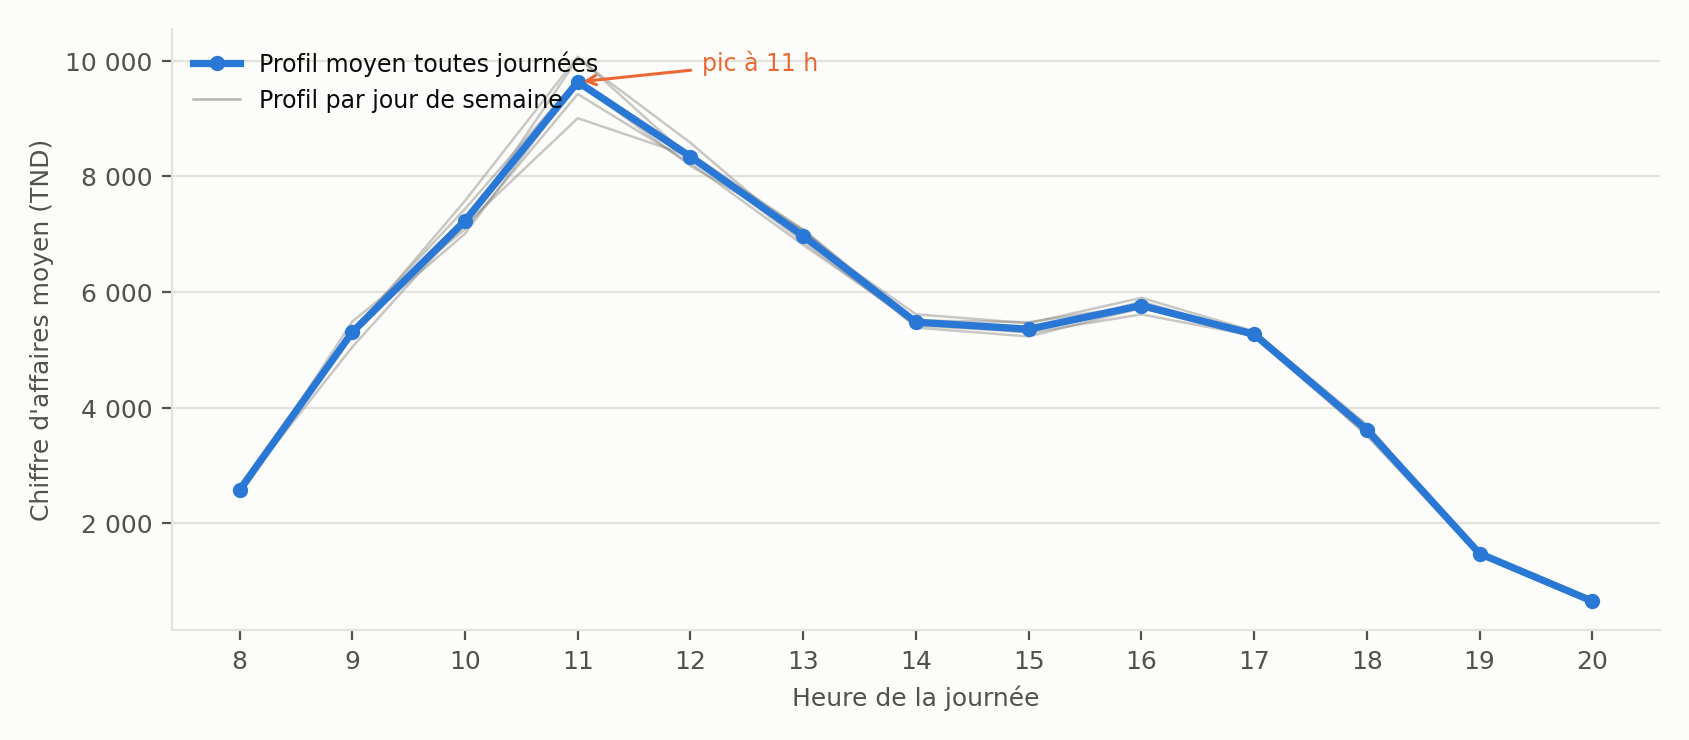
\includegraphics[width=\textwidth]{img/fig_profil_horaire.png}
    \caption{Profil intra-journalier moyen du chiffre d'affaires, par heure d'ouverture}
    \label{fig:profil-horaire-chap3}
\end{figure}

Le profil observé est nettement structuré et non uniforme, ce qui valide l'hypothèse sous-jacente à OD-2. Il présente deux régimes distincts séparés par une dépression de milieu de journée. Cette forme a une conséquence de conception importante : un seuil d'alerte exprimé en pourcentage constant de l'objectif journalier produirait un nombre d'alertes considérable en début de journée, où le cumulé est structurellement faible, et n'en produirait presque aucune en fin de journée. La détection d'anomalies devra donc comparer le réalisé au profil attendu \textit{à la même heure}, et non à une fraction linéaire de l'objectif. Ce choix, dicté par l'exploration, sera formalisé au chapitre~\ref{chap:modelisation}.

Le profil varie par ailleurs selon le jour de la semaine, ce qui impose d'apprendre non pas un profil unique mais sept profils, un par jour de semaine. Cette exigence multiplie par sept la quantité d'historique nécessaire pour estimer chaque profil avec une précision donnée, ce qui explique que le calcul soit restreint aux points de vente dont l'historique dépasse un seuil de couverture.

\subsection{Saisonnalité hebdomadaire}

L'objectif OD-1 suppose l'existence d'une saisonnalité hebdomadaire suffisamment marquée pour être exploitée par un modèle de série temporelle. La figure~\ref{fig:saisonnalite-hebdo-chap3} présente la distribution du chiffre d'affaires journalier par jour de semaine.

\begin{figure}[H]
    \centering
    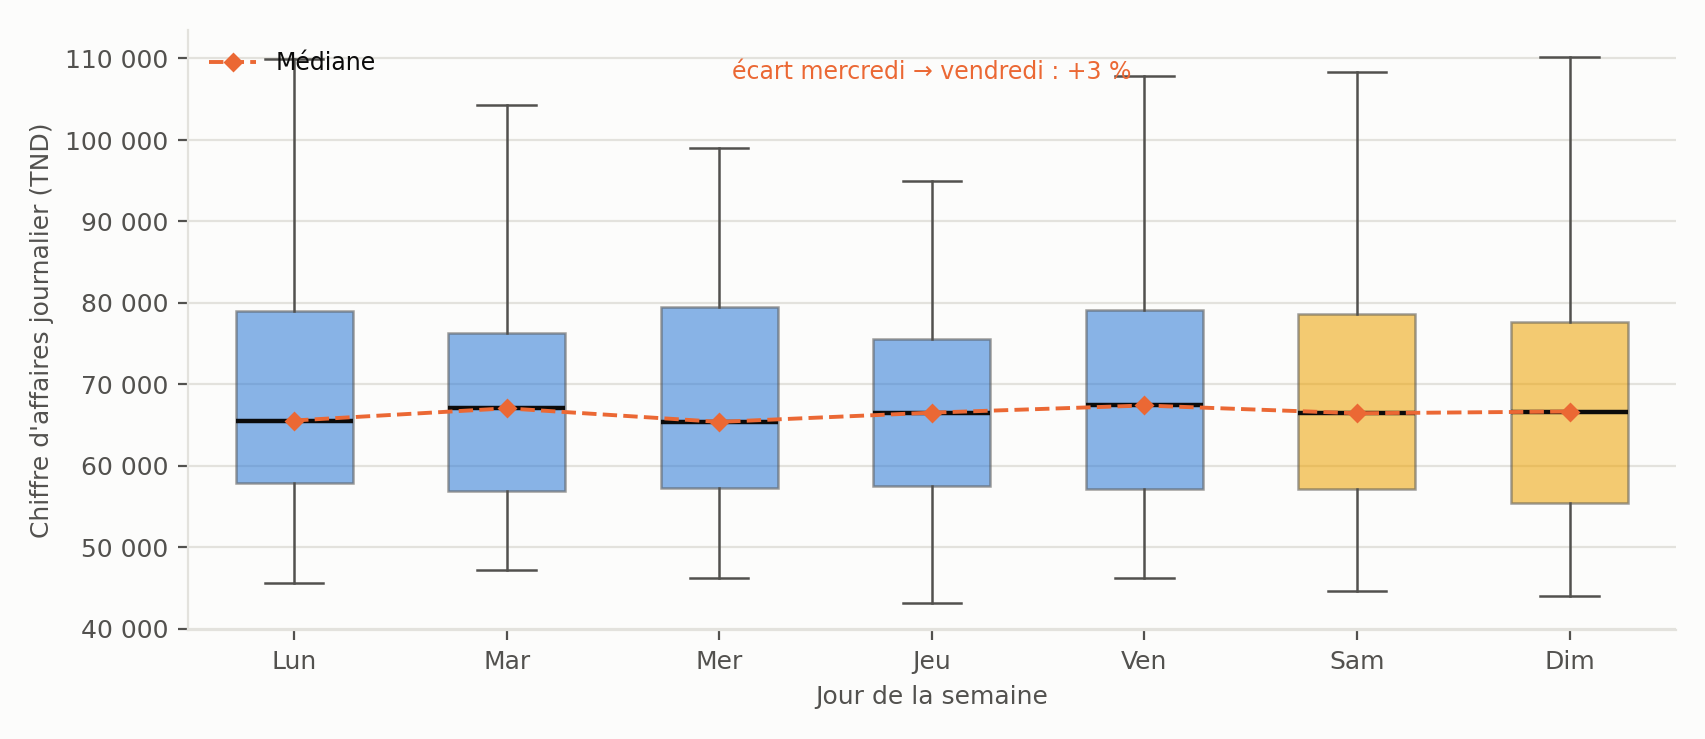
\includegraphics[width=\textwidth]{img/fig_saisonnalite_hebdo.png}
    \caption{Distribution du chiffre d'affaires journalier par jour de semaine}
    \label{fig:saisonnalite-hebdo-chap3}
\end{figure}

L'écart entre le jour le plus faible et le jour le plus fort est substantiel et systématique sur l'ensemble de la période, ce qui confirme la présence d'une composante hebdomadaire robuste. Cette observation justifie le choix, au chapitre~\ref{chap:modelisation}, d'une période saisonnière de sept jours pour le moteur statistique, et l'inclusion du jour de semaine comme variable explicative du modèle appris.

L'exploration révèle en revanche que l'amplitude de cette saisonnalité varie fortement d'un point de vente à l'autre. Un modèle unique, estimé sur l'ensemble du réseau, lisserait ces différences et dégraderait la prévision des points de vente atypiques. Un modèle par point de vente, à l'inverse, disposerait de peu de données pour les points de vente à faible volume. Cette tension est exactement celle que résout un modèle appris global prenant l'identifiant du point de vente comme variable explicative : il partage l'information entre points de vente tout en autorisant des comportements différenciés. Ce raisonnement fonde le choix de modélisation exposé en section~\ref{sec:modele-ca} du chapitre suivant.

\subsection{Concentration du catalogue}

Les objectifs OD-3 et OD-5 portent sur la maille de la référence produit. Leur faisabilité dépend directement de la distribution du volume de ventes sur le catalogue. La figure~\ref{fig:pareto-chap3} présente la courbe de concentration cumulée.

\begin{figure}[H]
    \centering
    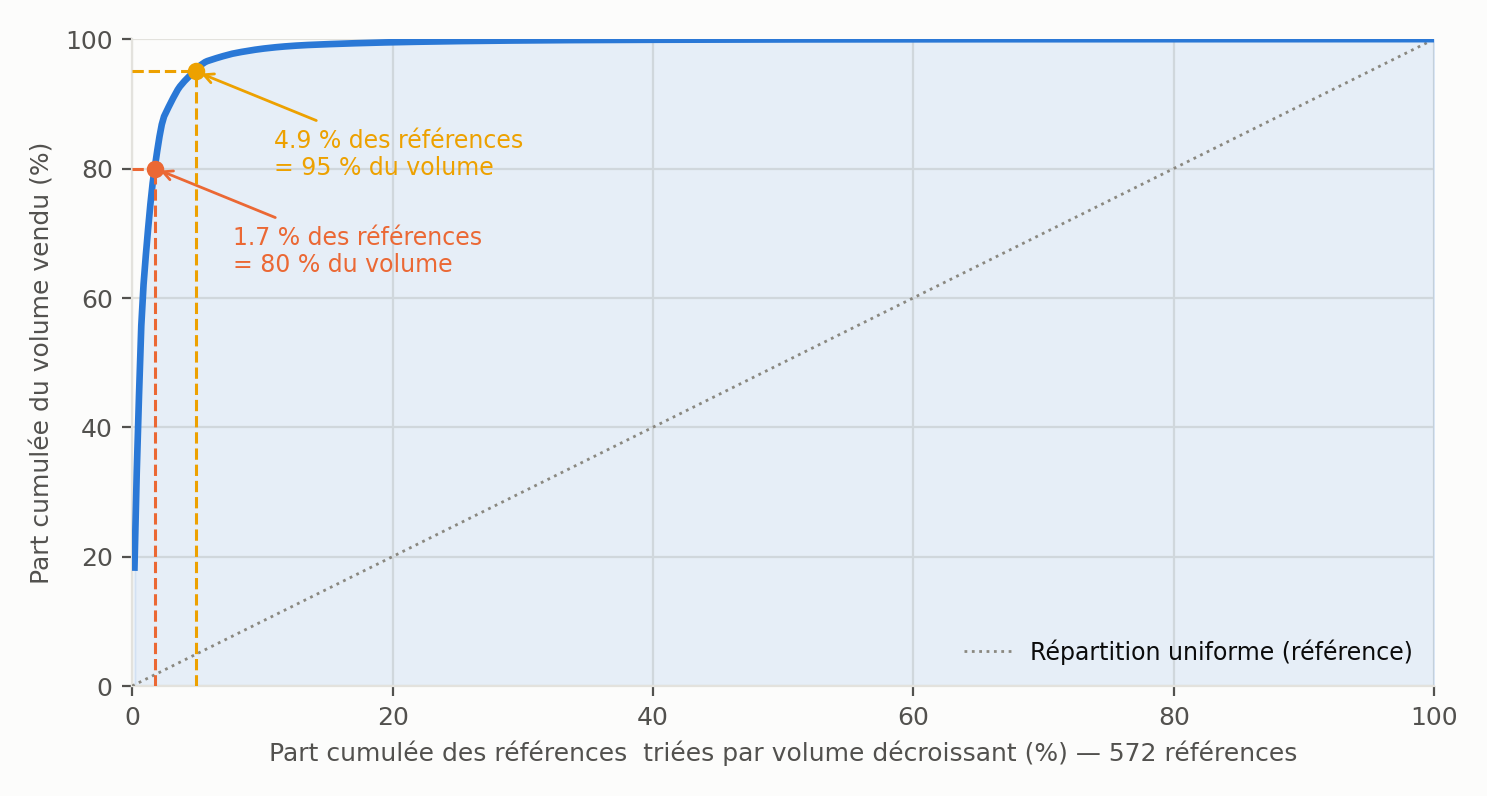
\includegraphics[width=0.86\textwidth]{img/fig_pareto_references.png}
    \caption{Concentration du volume de ventes sur le catalogue produit}
    \label{fig:pareto-chap3}
\end{figure}

La concentration est bien plus prononcée que ce que la formulation courante de la loi de Pareto laisse attendre \cite{silver2016inventory}. Sur les 572 références effectivement vendues, \textbf{1,7 \% suffisent à représenter 80 \% du volume} et 4,9 \% en représentent 95 \%. Autrement dit, une dizaine de références portent les quatre cinquièmes de l'activité, tandis que la quasi-totalité du catalogue vendu se répartit le cinquième restant. La courbe est si abrupte qu'elle atteint son plateau avant le dixième de l'axe des abscisses.

Cette observation a une conséquence méthodologique majeure, et c'est le premier point où l'exploration a conduit à réviser un objectif. Formulé au chapitre~\ref{chap:comprehension-metier}, l'objectif OD-3 visait la prévision de la demande « par référence », sans restriction. L'exploration montre qu'une telle prévision est dépourvue de sens pour la longue traîne : une référence vendue trois fois en vingt-deux mois ne porte aucune saisonnalité estimable, et toute prévision produite pour elle serait un artefact. Le périmètre d'OD-3 a donc été resserré aux couples référence et point de vente disposant d'au moins quatre-vingt-dix jours d'historique de ventes, seuil en deçà duquel l'estimation d'une composante hebdomadaire n'est pas défendable. Sur les 4 326 couples présents dans l'historique agrégé, \textbf{1 978 franchissent ce seuil}, soit 45,7 \% : c'est le périmètre effectif de la prévision de demande. Les couples exclus ne sont pas abandonnés pour autant : ils relèvent d'une logique de seuil de réapprovisionnement simple, décrite au chapitre~\ref{chap:modelisation}, et non d'une logique de prévision.

Ce chiffre appelle une remarque de lucidité. Un système qui annoncerait « prévision de la demande sur l'ensemble du catalogue » alors que moins de la moitié des couples dispose d'un historique exploitable ne serait pas faux sur la méthode, mais trompeur sur la portée. Le chapitre~\ref{chap:deploiement} montrera que cette limite est rendue visible jusque dans l'interface, chaque recommandation indiquant l'étage de la cascade de prévision dont elle provient.

\subsection{Distribution de la couverture de stock}

L'objectif OD-4 demande de classer chaque référence par niveau de risque. La grandeur pivot de cette classification est la couverture, c'est-à-dire le nombre de jours pendant lesquels le stock disponible peut absorber la demande attendue. La figure~\ref{fig:couverture-chap3} en présente la distribution.

\begin{figure}[H]
    \centering
    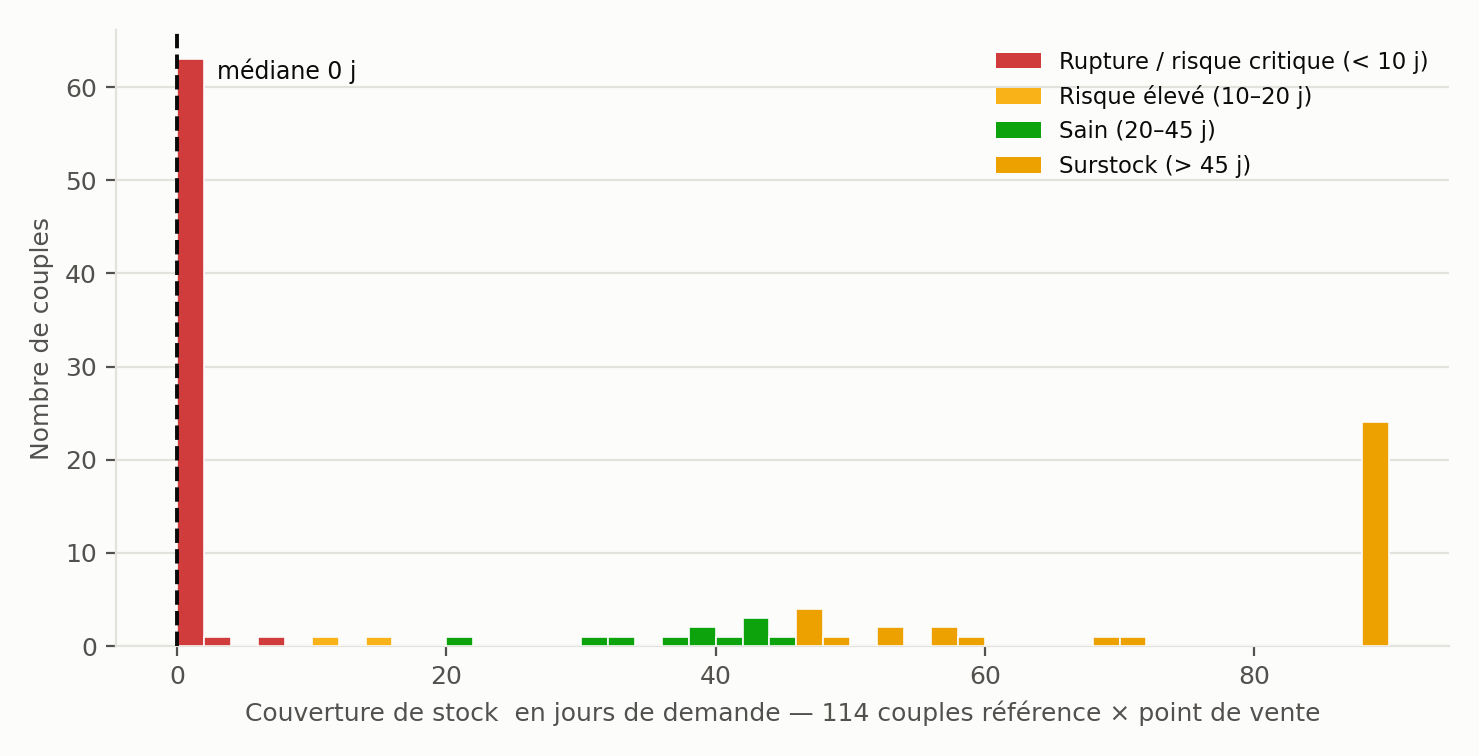
\includegraphics[width=0.86\textwidth]{img/fig_distribution_couverture.png}
    \caption{Distribution de la couverture de stock, en jours de demande}
    \label{fig:couverture-chap3}
\end{figure}

La distribution est fortement asymétrique et bimodale. Un premier mode rassemble les références à couverture très faible, qui constituent le gisement d'alertes de rupture. Un second mode, beaucoup plus étalé, rassemble des références dont la couverture dépasse largement l'horizon de réapprovisionnement, et qui relèvent d'une problématique de surstock -- immobilisation de trésorerie et risque d'obsolescence -- plutôt que de rupture.

Cette bimodalité justifie que la classification du risque de l'objectif OD-4 ne soit pas une simple échelle ordonnée à un seul sens de gravité, mais comporte deux extrémités problématiques. Elle justifie également la présence, dans l'arbre de décision du chapitre~\ref{chap:modelisation}, d'une branche de maintien qui recommande explicitement de \textit{ne pas} commander, décision qu'un système ne raisonnant que sur le risque de rupture ne saurait jamais formuler.

\subsection{Corrélations entre domaines}

L'objectif OD-6 postule qu'il existe un intérêt à croiser l'information de vente et l'information de stock pour hiérarchiser les produits à proposer. La figure~\ref{fig:correlation-chap3} présente la matrice de corrélation entre les grandeurs candidates à ce croisement.

\begin{figure}[H]
    \centering
    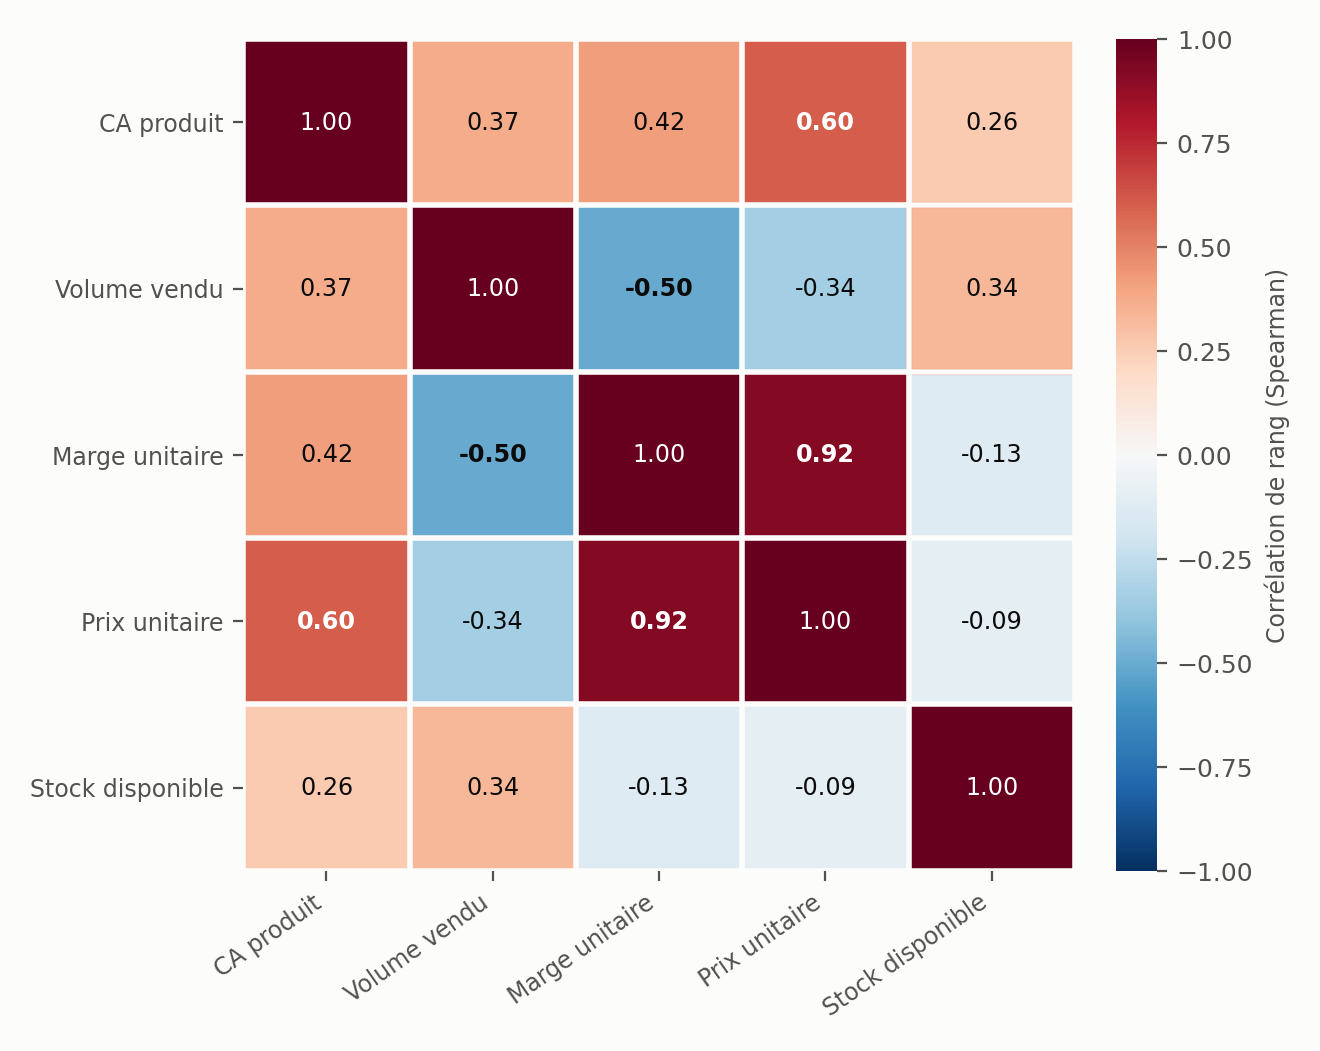
\includegraphics[width=0.82\textwidth]{img/fig_matrice_correlation.png}
    \caption{Corrélations entre grandeurs de vente, de stock et de contexte}
    \label{fig:correlation-chap3}
\end{figure}

Le résultat le plus instructif de cette matrice est une \textit{absence} de corrélation forte. La disponibilité en stock et le potentiel commercial d'une référence sont largement décorrélés : un produit à forte marge et fortement demandé n'est pas systématiquement bien approvisionné, et un produit abondamment stocké n'est pas nécessairement celui qu'il est pertinent de proposer. C'est précisément cette décorrélation qui donne sa valeur à l'objectif OD-6. Si les deux grandeurs avaient été fortement corrélées, un classement par la seule marge aurait suffi et le croisement inter-domaines n'aurait apporté aucune information. L'exploration confirme donc, par l'absence de redondance, la pertinence du score multicritère qui sera construit au chapitre~\ref{chap:modelisation}.

% ------------------------------------------------------------
\section{Vérification de la qualité des données}
\label{sec:qualite}
% ------------------------------------------------------------

\subsection{Méthode de vérification}

La vérification de la qualité a été conduite par introspection directe du catalogue de la base -- structure des colonnes, contraintes déclarées, index existants -- complétée de comptages et d'agrégats exécutés sur les données réelles. Ce choix mérite d'être explicité car il s'oppose à une pratique fréquente qui consiste à décrire le schéma d'après les fichiers de définition. Ces fichiers décrivent l'état \textit{voulu} ; l'introspection décrit l'état \textit{réel}. L'écart entre les deux a d'ailleurs été constaté au début du projet et a motivé une refonte complète du mécanisme de versionnement décrite en section~\ref{sec:versionnement}.

\subsection{Anomalies constatées et traitement retenu}

Le tableau~\ref{tab:qualite-chap3} recense les anomalies relevées, l'objectif analytique que chacune menace et le traitement retenu. Ce tableau constitue le livrable central de la tâche de vérification de la qualité au sens de CRISP-DM.

\begingroup
\setlength{\tabcolsep}{3pt}
\renewcommand{\arraystretch}{1.15}
\small

\begin{longtable}{|P{3.9cm}|P{1.9cm}|P{4.1cm}|P{4.1cm}|}
\hline
\rowcolor{red!75}
\textcolor{white}{\textbf{Anomalie constatée}} &
\textcolor{white}{\textbf{Objectif menacé}} &
\textcolor{white}{\textbf{Effet si non traitée}} &
\textcolor{white}{\textbf{Traitement retenu}} \\
\hline
\endhead
\hline
\endfoot
\hline
\endlastfoot
Attributs calendaires non renseignés dans les ventes agrégées & OD-3 & Profil saisonnier entièrement neutralisé : toute référence apparaît sans saisonnalité & Correction du calcul à la source ; recalcul des attributs à partir de la date \\
\hline
Longue traîne de références à historique insuffisant & OD-3, OD-5 & Prévisions produites sur du bruit, sans valeur décisionnelle & Seuil d'inclusion de 90 jours d'historique ; repli sur règle de seuil pour les exclues \\
\hline
Absence de clé étrangère sur l'identifiant produit du flux temps réel & OD-1, OD-6 & Recommandation possible sur une référence inexistante & Contrôle applicatif de cohérence ; contrainte différée pour préserver la tolérance du flux \\
\hline
Réceptions de commande non tracées dans les mouvements de stock & OD-5 & Chaîne causale incomplète : impossible de mesurer l'effet d'une décision & Écriture du mouvement à la transition de réception ; migration dédiée \\
\hline
Identifiant d'exécution d'agent non renseigné sur les alertes & OD-8 & Impossibilité de rattacher une alerte au cycle qui l'a produite & Propagation de l'identifiant dans le contrat de retour de l'orchestrateur \\
\hline
Paramètres logistiques laissés à leur valeur par défaut & OD-5 & Quantités recommandées justes en méthode mais fausses en valeur & Limite assumée et documentée ; sensibilité mesurée au chapitre~\ref{chap:evaluation} \\
\hline
Tables héritées sans données ni usage & aucun & Confusion de lecture, coût de maintenance & Suppression après vérification d'absence d'usage \\
\hline
Absence de contraintes d'intégrité entre domaines & OD-4, OD-5 & Recommandations orphelines de tout référentiel & Ajout de clés étrangères et de contraintes de validité \\
\hline
Duplication possible de recommandations en attente & OD-5 & Propositions concurrentes sur le même couple & Index unique partiel sur les recommandations en attente \\
\hline
\caption{Anomalies de qualité, objectifs menacés et traitements retenus}
\label{tab:qualite-chap3}
\end{longtable}
\endgroup

Deux anomalies de cette liste méritent un développement, car elles illustrent deux natures de défaut très différentes.

La première est celle des \textbf{attributs calendaires non renseignés}. Il s'agissait d'un défaut silencieux : aucune erreur n'était levée, aucun traitement n'échouait, et les tables se remplissaient normalement. Le défaut ne se manifestait que par une propriété statistique aberrante -- toutes les références présentaient une saisonnalité hebdomadaire nulle, ce qui est empiriquement impossible au vu de la figure~\ref{fig:saisonnalite-hebdo-chap3}. C'est l'exploration, et non un contrôle technique, qui a permis de le détecter. Ce cas illustre pourquoi la phase de compréhension des données ne peut être réduite à une vérification d'intégrité automatisée : certaines anomalies ne sont visibles qu'à la lumière d'une attente métier.

La seconde est celle des \textbf{paramètres logistiques par défaut}. Elle ne se corrige pas techniquement : la donnée manquante n'existe nulle part, elle n'a jamais été saisie. Le seul traitement honnête consiste à documenter la limite et à en mesurer l'effet. C'est le parti retenu : les quantités recommandées sont calculées avec la méthode correcte sur des paramètres partiellement approximatifs, et le chapitre~\ref{chap:evaluation} distingue explicitement l'erreur de méthode de l'erreur de paramétrage. Présenter ce système comme produisant des quantités exactes serait une faute méthodologique.

\subsection{Contraintes d'intégrité mises en place}

Le traitement des anomalies a conduit à durcir le modèle physique. Sept clés étrangères ont été ajoutées pour rattacher les tables opérationnelles -- alertes, recommandations, bons de commande, mouvements de stock -- aux trois référentiels centraux. Des contraintes de validité ont été posées sur les colonnes de statut, afin qu'aucune valeur hors nomenclature ne puisse être écrite. Un index unique partiel garantit qu'une seule recommandation en attente peut exister à un instant donné pour un couple référence et point de vente, ce qui évite que deux cycles d'agents concurrents ne produisent des propositions contradictoires.

Une opération de nettoyage structurel a par ailleurs été menée : vingt-sept tables héritées, dépourvues de données et d'usage, ont été supprimées après vérification, faisant passer la base de soixante-dix-sept à cinquante tables. Cette opération n'améliore aucune métrique de modèle, mais elle réduit substantiellement le coût de compréhension de la base -- ce qui est, dans un projet de fin d'études destiné à être repris, une forme de qualité à part entière.

Un dernier point mérite d'être signalé car il relève d'une correction de fond. Un déclencheur de base de données mettait à jour le stock physique à la création d'une recommandation, avant toute approbation humaine. Une simple \textit{proposition} de commande gonflait donc le stock réel, faussant en cascade la couverture, la classification du risque et les recommandations suivantes. Ce déclencheur a été supprimé. L'incident illustre un principe qui sera repris au chapitre~\ref{chap:modelisation} : une suggestion n'est pas un fait, et rien de ce que le système propose ne doit modifier l'état du monde avant validation humaine.

% ------------------------------------------------------------
\section{Préparation des données}
\label{sec:preparation}
% ------------------------------------------------------------

La phase de préparation transforme les sources vérifiées en jeux de données directement consommables par les modèles. CRISP-DM la décompose en cinq tâches, traitées ci-dessous dans l'ordre. La figure~\ref{fig:pipeline-preparation-chap3} donne la vue d'ensemble du pipeline construit.

\begin{figure}[H]
    \centering
    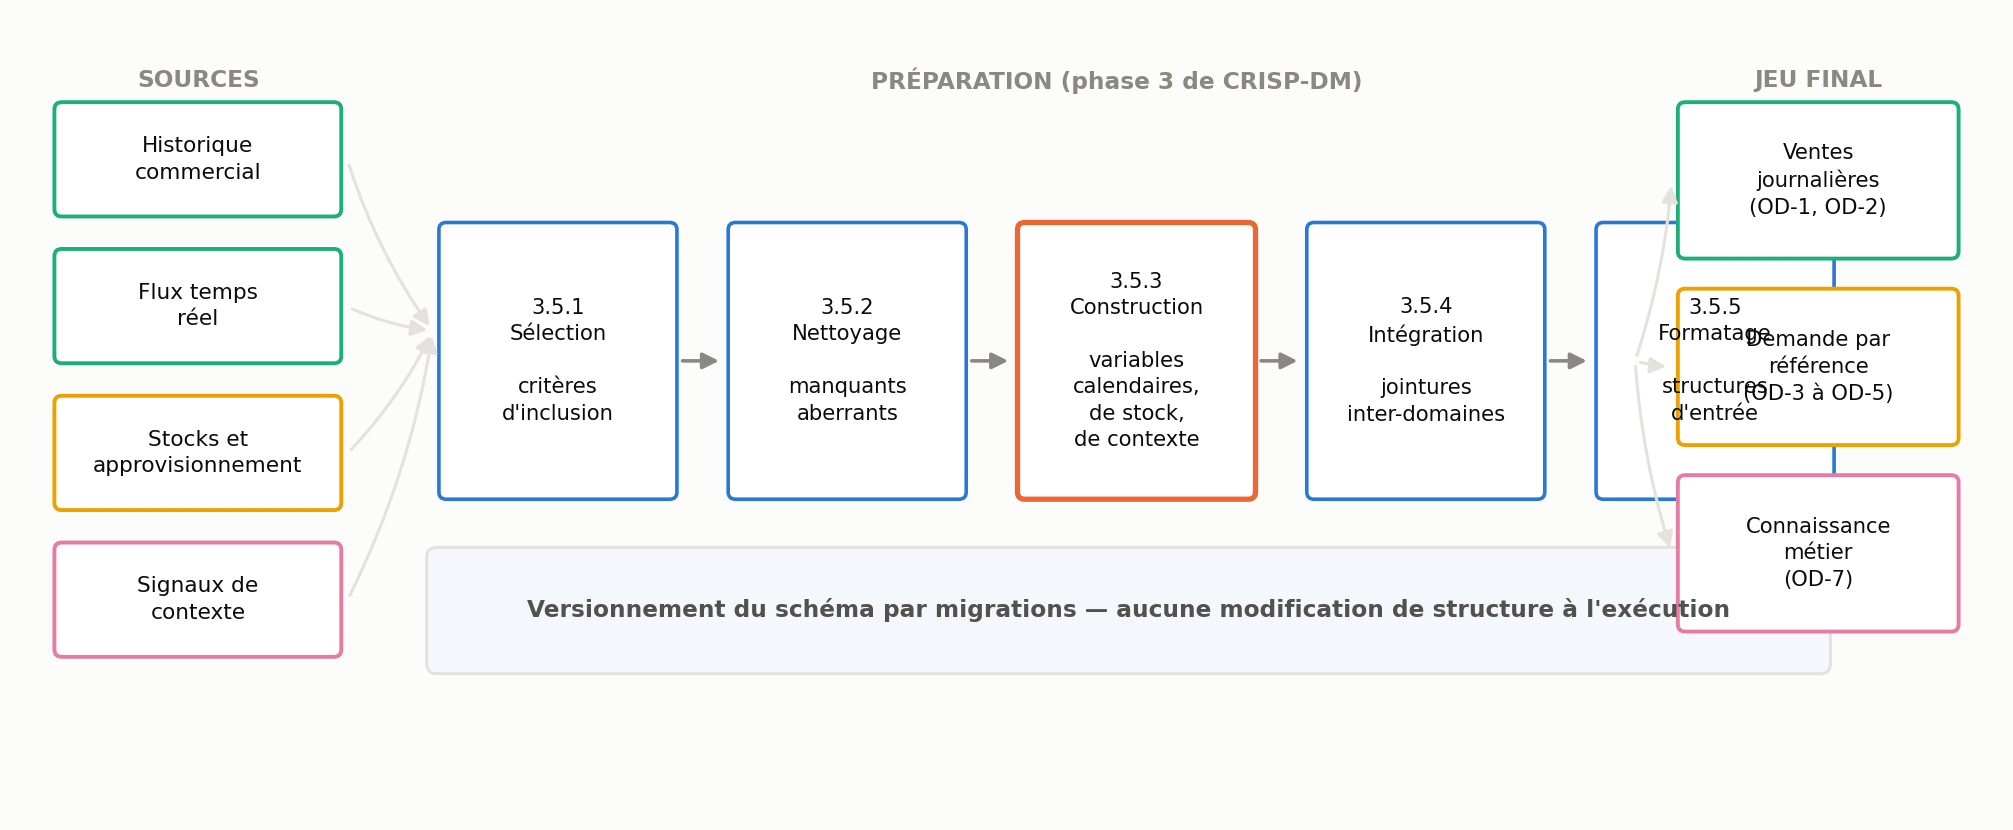
\includegraphics[width=\textwidth]{img/fig_pipeline_preparation.png}
    \caption{Pipeline de préparation des données, de la source au jeu d'entrée des modèles}
    \label{fig:pipeline-preparation-chap3}
\end{figure}

\subsection{Sélection des données}

La sélection retient, pour chaque objectif, le sous-ensemble pertinent selon des critères explicites.

Pour la prévision du chiffre d'affaires (OD-1), l'unité d'observation est le couple point de vente et jour. Sont retenus les points de vente présentant une activité continue sur la fenêtre d'apprentissage, à l'exclusion de ceux dont l'historique comporte des interruptions prolongées qui traduisent une fermeture ou un défaut de remontée plutôt qu'une absence de vente. Le panel ainsi constitué compte cent cinquante et un points de vente et près de quatre-vingt-dix-huit mille observations jour-boutique.

Pour la prévision de la demande (OD-3), l'unité d'observation est le triplet référence, point de vente et jour. Le critère d'inclusion est le seuil de quatre-vingt-dix jours d'historique justifié en section~\ref{sec:exploration}. Une garantie complémentaire a été ajoutée à ce critère : certains points de vente à faible volume, bien qu'éligibles, se trouvaient systématiquement écartés par la sélection des couples les plus actifs. Une liste d'inclusion explicite garantit désormais leur présence, faute de quoi ces points de vente auraient été durablement privés de prévision -- un biais de sélection d'autant plus insidieux qu'il n'aurait produit aucune erreur visible.

Pour la détection d'anomalies horaires (OD-2), la sélection porte sur les journées complètes uniquement : une journée partiellement remontée produirait des écarts horaires artificiels en fin de journée.

\subsection{Nettoyage des données}

Le nettoyage applique les traitements arrêtés au tableau~\ref{tab:qualite-chap3}. Trois familles de règles ont été retenues.

Les \textbf{valeurs manquantes} sont traitées différemment selon leur nature. Pour les grandeurs observées, une valeur manquante sur une journée d'ouverture est interprétée comme une absence de vente et remplacée par zéro, tandis qu'une valeur manquante sur une journée de fermeture conduit à exclure l'observation : confondre les deux cas apprendrait au modèle qu'il se vend zéro les jours fériés, alors qu'il ne se vend rien parce que la boutique est fermée. Pour les paramètres de gestion, une valeur manquante est remplacée par une valeur de repli explicite et tracée comme telle, afin que le chapitre~\ref{chap:evaluation} puisse distinguer les décisions fondées sur des paramètres réels de celles fondées sur des valeurs par défaut. Pour les signaux externes, une valeur manquante est imputée par la médiane historique de la même période, cette médiane étant précalculée et figée pour garantir la reproductibilité.

Les \textbf{valeurs aberrantes} font l'objet d'un traitement volontairement conservateur. Une journée de chiffre d'affaires exceptionnellement élevée est le plus souvent un fait réel -- lancement d'un terminal, opération commerciale -- et non une erreur de saisie. L'écrêtage systématique aurait détruit précisément le signal que les variables de contexte doivent expliquer. Seules sont écartées les valeurs incohérentes au sens strict : quantités négatives, montants nuls associés à une quantité non nulle, horodatages hors plage d'ouverture.

La \textbf{déduplication} s'appuie sur la clé naturelle de chaque table. Elle a principalement concerné les instantanés de stock, où une même journée pouvait faire l'objet de plusieurs remontées.

\subsection{Construction des variables}

La construction est la tâche qui apporte le plus de valeur analytique, car c'est elle qui encode la connaissance métier sous forme exploitable par un modèle. Le tableau~\ref{tab:variables-chap3} recense les familles de variables construites.

\begingroup
\setlength{\tabcolsep}{3pt}
\renewcommand{\arraystretch}{1.15}
\small

\begin{longtable}{|P{3.2cm}|P{5.6cm}|P{4.9cm}|}
\hline
\rowcolor{red!75}
\textcolor{white}{\textbf{Famille}} &
\textcolor{white}{\textbf{Variables construites}} &
\textcolor{white}{\textbf{Justification métier}} \\
\hline
\endhead
\hline
\endfoot
\hline
\endlastfoot
Calendaires & Jour de semaine, quantième du mois, mois, semaine, indicateurs de début et de fin de mois & Encodent les cycles de paie et les habitudes d'achat \\
\hline
Événementielles & Indicateur de jour férié, de fête religieuse, de période de Ramadan, de rentrée scolaire ; distance en jours à l'événement le plus proche & Capturent les effets calendaires que la saisonnalité hebdomadaire ne peut représenter \\
\hline
Historiques décalées & Ventes des jours précédents, moyennes mobiles à plusieurs fenêtres, moyenne du même jour de semaine & Fournissent au modèle appris la mémoire courte que le modèle statistique porte structurellement \\
\hline
Tendancielles & Pente locale, rapport entre moyenne courte et moyenne longue & Détectent les inflexions de tendance non encore visibles dans le niveau \\
\hline
Commerciales & Indicateur de promotion active, intensité de la promotion, rang de la référence dans les meilleures ventes & Expliquent les écarts de demande d'origine commerciale \\
\hline
De stock & Couverture en jours, rotation, indicateur de rupture récente & Alimentent la classification du risque et corrigent la demande observée en période de rupture \\
\hline
Contextuelles externes & Conditions météorologiques, proximité géographique d'un événement & Modulent la fréquentation du point de vente \\
\hline
\caption{Familles de variables construites et justification métier}
\label{tab:variables-chap3}
\end{longtable}
\endgroup

Une variable construite mérite un commentaire particulier : l'\textbf{indicateur de rupture récente}. Sa raison d'être est un biais classique et sévère de la prévision de demande en distribution. Ce que l'on observe n'est pas la demande mais les ventes, et les ventes sont bornées par le stock disponible. Une référence en rupture enregistre zéro vente, ce qu'un modèle naïf interprète comme une demande nulle, et pour laquelle il recommandera donc de ne pas réapprovisionner -- perpétuant la rupture. Signaler explicitement les périodes de rupture permet au modèle de traiter ces observations comme censurées plutôt que comme des demandes nulles. Cette variable ne corrige pas entièrement le biais, mais elle en limite considérablement la propagation.

\subsection{Intégration des données}

L'intégration réalise les jointures entre domaines. Trois rapprochements structurent le jeu final.

Le rapprochement \textbf{ventes et stock} s'effectue sur le couple référence et point de vente, à la maille journalière. Il permet de qualifier chaque observation de vente par l'état de stock qui l'accompagnait, condition nécessaire au traitement du biais de censure évoqué ci-dessus.

Le rapprochement \textbf{ventes et contexte} s'effectue sur la date et, pour les événements localisés, sur la proximité géographique entre le lieu de l'événement et les coordonnées du point de vente. Ce second critère est ce qui distingue un signal utile d'un signal dilué : un concert n'affecte pas uniformément le réseau national, mais les points de vente situés dans son voisinage.

Le rapprochement \textbf{ventes et objectifs} s'effectue sur le couple point de vente et date. Il est indispensable à la notion d'écart, elle-même au fondement du déclenchement des cycles de coaching.

Le principal piège rencontré lors de l'intégration a été une incohérence de nommage entre le flux temps réel et le référentiel produit : la colonne portant la référence produit n'y porte pas le même nom que dans l'historique et n'est reliée par aucune contrainte. La cohérence des valeurs a été vérifiée exhaustivement et s'est révélée totale, mais la contrainte n'a pas été posée afin de préserver la tolérance du flux entrant. Ce compromis est assumé et documenté : il échange une garantie structurelle contre une garantie de disponibilité, ce que la nature temps réel du flux justifie.

\subsection{Formatage}

Le formatage produit les structures d'entrée attendues par chaque famille de modèles : une série temporelle indexée par date pour le moteur statistique, une table de vecteurs de variables pour le modèle appris, une structure de documents découpés et vectorisés pour la recherche documentaire. Cette dernière est décrite au chapitre~\ref{chap:modelisation}, où elle relève pleinement de la modélisation.

Un point de conception mérite d'être souligné : la construction du vecteur de variables est assurée par un composant unique, partagé entre la chaîne d'apprentissage hors ligne et la chaîne de production. Ce choix élimine par construction la classe de défauts la plus difficile à diagnostiquer en apprentissage automatique, celle où l'entraînement et l'inférence ne calculent pas exactement la même variable sous le même nom -- défaut qui ne produit aucune erreur, seulement une dégradation silencieuse de la qualité des prévisions.

\subsection{Versionnement du schéma}
\label{sec:versionnement}

Une règle structurante a été posée et tenue sur l'ensemble du projet : \textbf{aucune modification de structure n'est effectuée à l'exécution}. Toute évolution du schéma passe par une migration numérotée, versionnée et rejouable, et l'application ne crée jamais de table à son démarrage.

Cette règle est une réponse directe à une situation constatée au début du projet : les fichiers de migration décrivaient un schéma différent de celui réellement en production, tandis que des instructions de création de tables subsistaient dans le code applicatif. La structure réelle de la base n'était alors documentée nulle part de façon fiable, ce qui rendait toute reprise du projet hasardeuse. La refonte a consisté à reconstituer une ligne de migrations unique, à partir d'un socle reflétant l'état réel, puis à y enchaîner les évolutions successives -- dix-huit migrations à ce jour. Chacune des corrections de qualité recensées au tableau~\ref{tab:qualite-chap3} correspond à une migration identifiée.

Ce point peut sembler relever de l'ingénierie logicielle plutôt que de la science des données. Il relève en réalité pleinement de la préparation des données au sens de CRISP-DM : la reproductibilité du jeu de données final est une propriété du processus qui le produit, et un jeu de données que l'on ne sait pas reconstruire n'est pas un livrable, c'est un artefact.

% ------------------------------------------------------------
\section{Jeu de données final et protocole de découpage}
\label{sec:jeu-final}
% ------------------------------------------------------------

\subsection{Description du jeu de données final}

Le jeu de données final se compose de trois ensembles cohérents, correspondant aux trois familles d'objectifs analytiques.

L'ensemble \textbf{ventes journalières} porte sur cent cinquante et un points de vente et couvre la période d'octobre 2024 à juillet 2026, soit près de quatre-vingt-dix-huit mille observations jour-boutique, chacune décrite par les variables calendaires, événementielles, historiques décalées et tendancielles du tableau~\ref{tab:variables-chap3}. Il sert les objectifs OD-1 et OD-2.

L'ensemble \textbf{demande par référence} porte sur les couples référence et point de vente franchissant le seuil d'historique, soit un peu plus de quatre mille couples, à la maille journalière, enrichis des variables commerciales, de stock et contextuelles. Il sert les objectifs OD-3 à OD-5.

L'ensemble \textbf{connaissance métier} rassemble les documents textuels -- argumentaires, scripts de vente, procédures, fiches produit -- découpés et vectorisés. Il sert l'objectif OD-7.

\subsection{Protocole de découpage temporel}

Le découpage entre apprentissage, validation et test obéit à une contrainte non négociable en prévision : il doit être \textbf{strictement chronologique}. Un découpage aléatoire placerait dans l'ensemble d'apprentissage des observations postérieures à celles de l'ensemble de test, permettant au modèle d'utiliser une information future pour prédire le passé. Cette fuite produit des performances excellentes en évaluation et sans valeur en production. La figure~\ref{fig:decoupage-chap3} illustre le protocole retenu.

\begin{figure}[H]
    \centering
    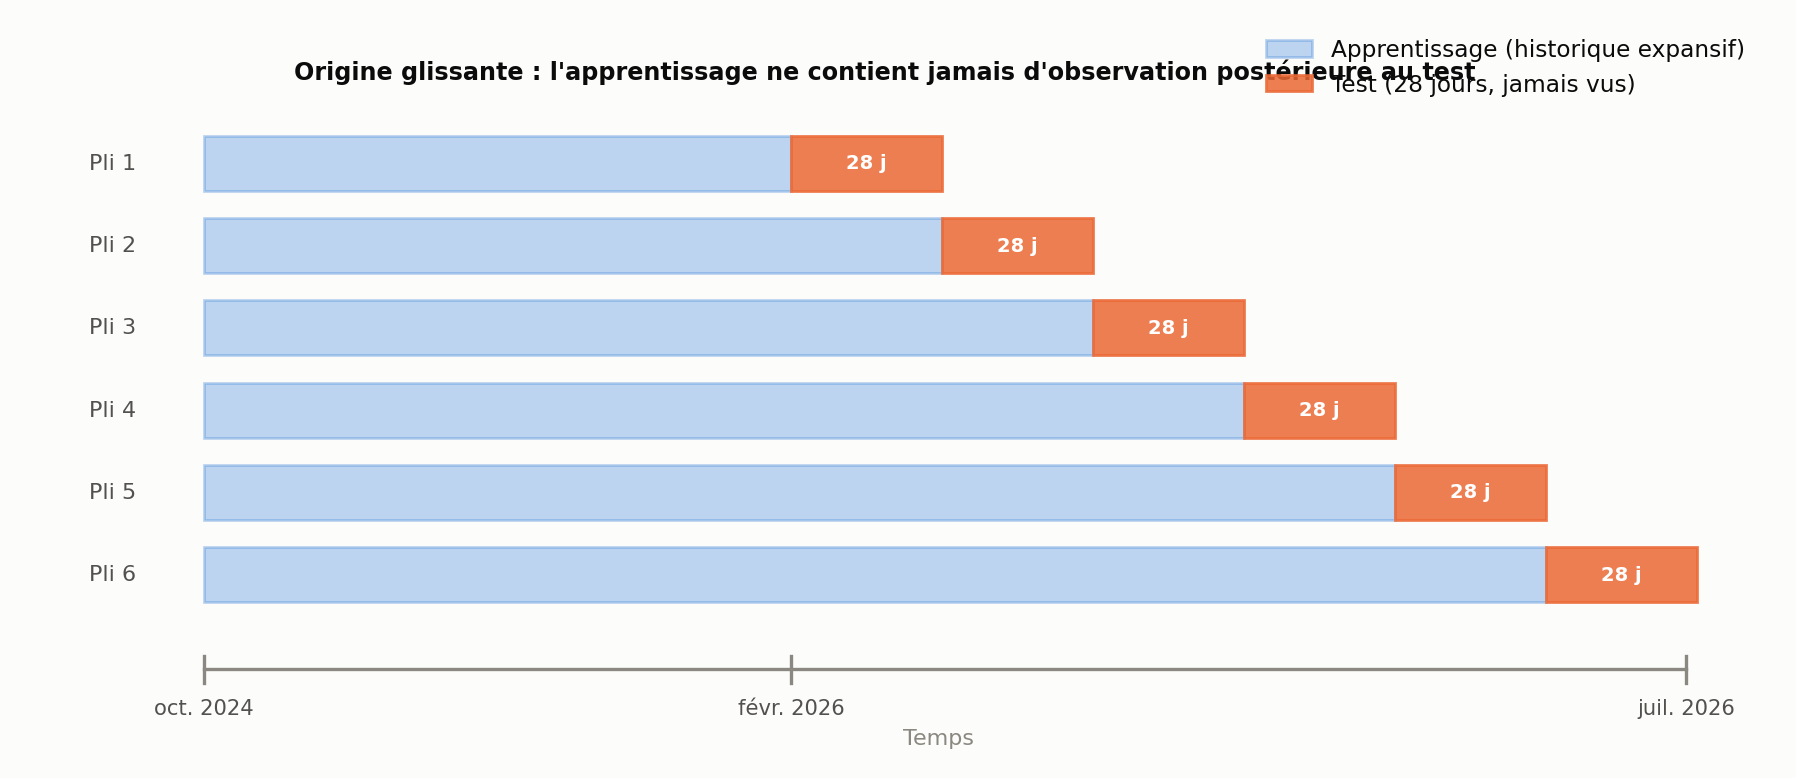
\includegraphics[width=\textwidth]{img/fig_decoupage_temporel.png}
    \caption{Protocole de découpage temporel à origine glissante}
    \label{fig:decoupage-chap3}
\end{figure}

Le protocole retenu est le rétro-test à origine glissante, recommandé par la littérature de référence en prévision \cite{hyndman2021fpp}. Il consiste à répéter l'opération suivante : entraîner le modèle sur toutes les données antérieures à une date d'origine, évaluer sur la fenêtre qui suit immédiatement cette origine, puis avancer l'origine et recommencer. Six plis successifs de vingt-huit jours ont été constitués, chacun entraîné sur l'historique expansif qui le précède.

Ce protocole présente deux avantages décisifs sur un simple découpage en deux blocs. D'une part, il évalue le modèle sur six fenêtres temporelles distinctes plutôt qu'une seule, ce qui évite qu'une conclusion ne repose sur les particularités d'une unique période. D'autre part, il reproduit fidèlement les conditions réelles d'exploitation : en production, le modèle est toujours entraîné sur tout le passé disponible et prédit l'avenir immédiat. Les résultats obtenus sous ce protocole sont donc directement transposables, ce que le chapitre~\ref{chap:evaluation} exploitera.

Une précaution complémentaire a été prise sur les variables construites. Toute variable décalée, moyenne mobile ou statistique agrégée est calculée exclusivement à partir d'observations antérieures à la date de la prédiction. Cette précaution paraît évidente énoncée ainsi, mais elle est la source la plus fréquente de fuite involontaire : une moyenne calculée sur l'ensemble de la période, puis jointe à chaque observation, injecte de l'information future dans chaque ligne sans qu'aucun découpage ne le signale.

% ------------------------------------------------------------
\section*{Conclusion}
\addcontentsline{toc}{section}{Conclusion}
% ------------------------------------------------------------

Ce chapitre a conduit les deuxième et troisième phases de CRISP-DM. La collecte a réuni quatre familles de sources en une base unique de cinquante et une tables organisées en neuf domaines métier, portant près de deux millions de lignes de transactions sur vingt-deux mois. La description a établi le dictionnaire des attributs structurants et le modèle relationnel, en distinguant les données observées des paramètres de gestion -- distinction dont la portée sur l'évaluation a été soulignée.

L'exploration a rempli sa fonction méthodologique : valider ou invalider les hypothèses implicites des objectifs analytiques. Elle a confirmé l'existence d'un profil intra-journalier structuré et d'une saisonnalité hebdomadaire robuste, validant OD-2 et OD-1. Elle a en revanche conduit à resserrer le périmètre d'OD-3, la concentration extrême du catalogue rendant la prévision individuelle dépourvue de sens sur la longue traîne. Elle a enfin confirmé, par l'absence de corrélation entre disponibilité et potentiel commercial, la pertinence du croisement inter-domaines visé par OD-6.

La vérification de la qualité a recensé neuf anomalies, dont deux appellent une lecture particulière : un défaut silencieux d'attributs calendaires, détectable seulement à la lumière d'une attente métier, et une insuffisance de paramétrage logistique qui ne se corrige pas et dont l'effet est explicitement assumé. La préparation a ensuite produit les trois ensembles du jeu final, à partir d'un pipeline dont la reproductibilité est garantie par un versionnement strict du schéma et par le partage d'un composant unique de construction des variables entre apprentissage et production.

Le protocole de découpage à origine glissante, avec ses six plis chronologiques et sa règle d'antériorité stricte sur les variables construites, ferme le chapitre. Il fixe les conditions dans lesquelles toute performance annoncée au chapitre~\ref{chap:evaluation} devra avoir été obtenue.

\textbf{Décision de fin de phase.} Les données disponibles satisfont les prérequis des objectifs OD-1, OD-2, OD-4, OD-6 et OD-7 sans restriction. L'objectif OD-3 est retenu avec un périmètre resserré aux références disposant d'un historique suffisant. L'objectif OD-5 est retenu avec une réserve explicite sur la qualité du paramétrage logistique, dont l'effet sera mesuré séparément. Sous ces réserves, la phase de modélisation est autorisée : elle fait l'objet du chapitre suivant.
